\subsection{Inductances characterization}
\label{subsec:inductances_characterization}

A key parameter of the system is the inductance of the coils.

As already proposed in Equation \ref{eq:model_for_inductance}, the inductance of the coils cannot be considered constant and both its dependence on the current and the position of the ball must be taken into account when dealing with the magnetic levitation system.

In order to identify the inductance of the coils and all the parameters needed to characterize them, we have to measure the values of $L_1$ and $L_2$ for many currents and ball positions.
Once we have these values, we can fit the data to the model proposed in Equation \ref{eq:model_for_inductance} and identify the parameters.

Given a certain (fix in time) position of the ball and a certain current step input, we can measure the value of the inductance of the coils, knowing that:

\begin{equation}
    V = R I + \frac{d (L I)}{d t} = R I + \left( \frac{\partial L}{\partial I} I + L \right) \dot{I}
\end{equation}

If we suppose for a moment that the variation of the inductance with the current is negligible, we can obtain a closed form solution for the current in the RL circuit as follows:

\begin{equation}
    I(t) = \frac{V_{max}}{R_0} \left( 1 - e^{- \frac{R_0}{L_0} t} \right)
    \label{eq:current_in_rl_circuit}
\end{equation}

Given the previous equation, we can adopt the following strategy to fully characterize the inductance of the coils over the range of possible ball positions and currents:

\begin{enumerate}
    \item Fix the ball at a certain height ($z^*$);
    \item Apply a certain current step input to the system ($I^*$);
    \item Measure the current in the coils ($I(t)$);
    \item Fit the measured current to the model proposed in Equation \ref{eq:current_in_rl_circuit} and identify $L(z^*, I^*)$;
    \item Repeat from step 2 for different step inputs of currents;
    \item Repeat from step 1 for different ball positions.
\end{enumerate}

In Figure \ref{fig:inductance_characterization_currents} we can see on the left all the dynamics of the current in the coils for different step inputs of currents and different ball positions, while on the right we can see the fitting of the data to the model proposed in Equation \ref{eq:current_in_rl_circuit}.

\begin{figure}[H]
    \centering
    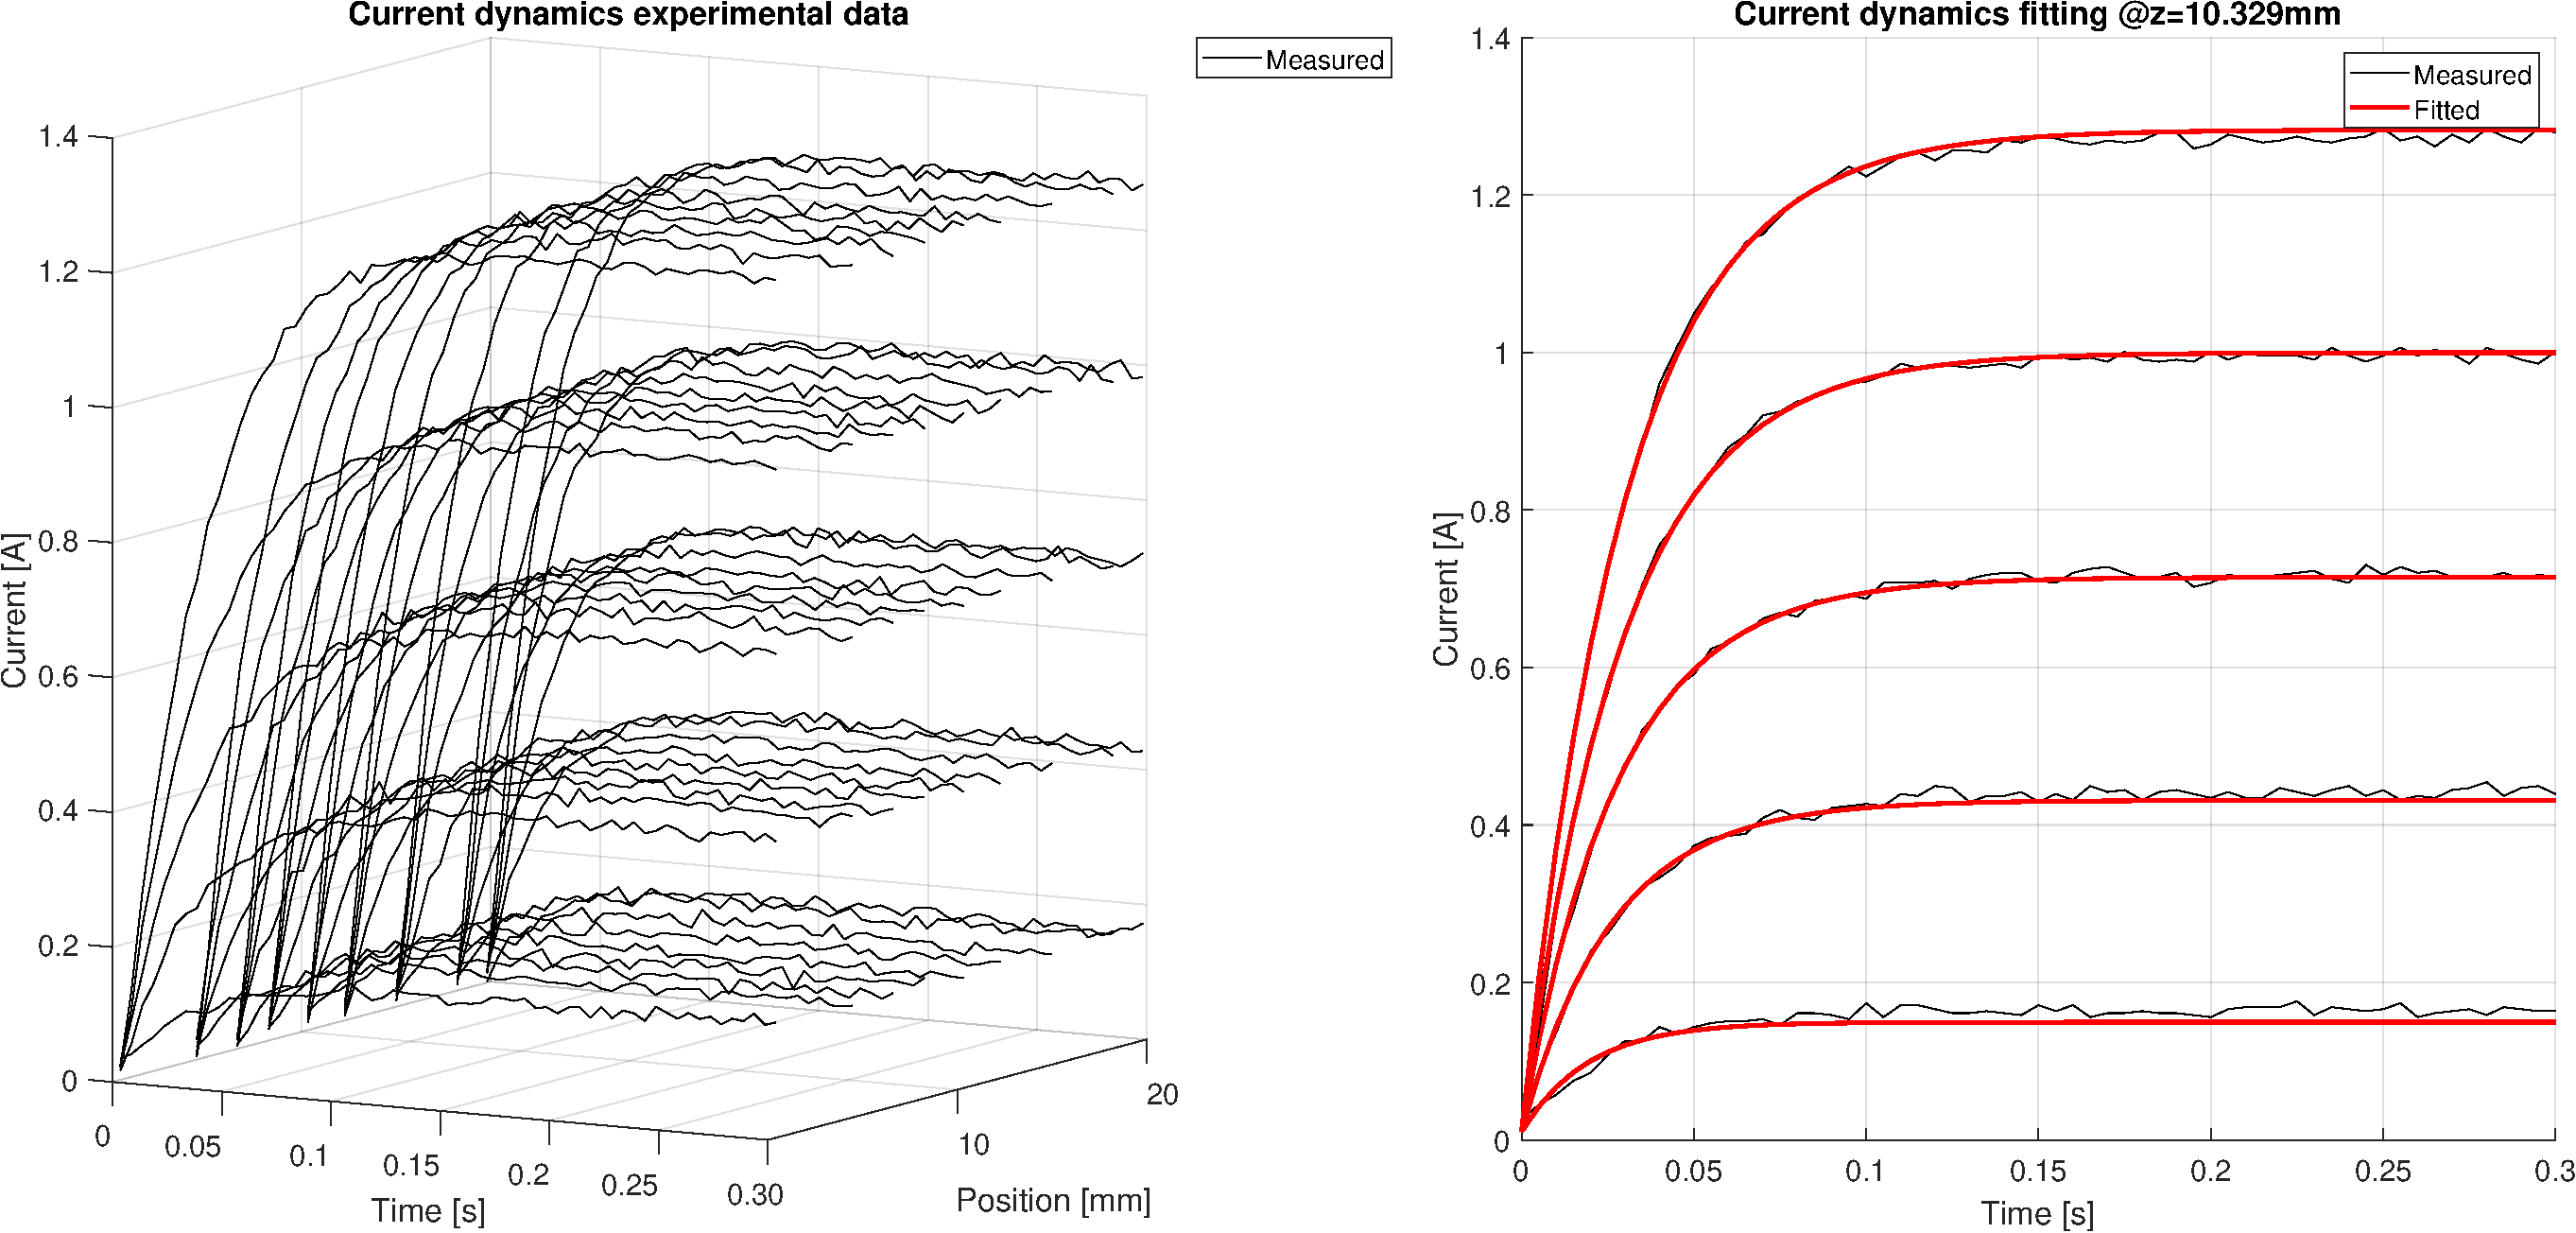
\includegraphics[width=1\textwidth]{img/MATLAB/identification/currents.pdf}
    \caption{Inductance characterization for different currents and ball positions}
    \label{fig:inductance_characterization_currents}
\end{figure}

From the right side of Figure \ref{fig:inductance_characterization_currents} we can see that the fitting of the data to the model proposed in Equation \ref{eq:current_in_rl_circuit} is optimal for middle values of the current, while it tends to underestimate and overestimate the current for low and high values of the current, respectively.
This behavior is probably due to the fact that the variation of the inductance with the current that has been neglected in the model of the current (Equation \ref{eq:current_in_rl_circuit}) is not negligible and should have been taken into account.

Thanks to the data obtained from the multiple tests, we can now fit the values of the inductance of the coils to the model proposed in Equation \ref{eq:model_for_inductance} and identify the parameters.
The obtained model fitting is shown in Figure \ref{fig:inductance_characterization_inductance}.

\begin{figure}[H]
    \centering
    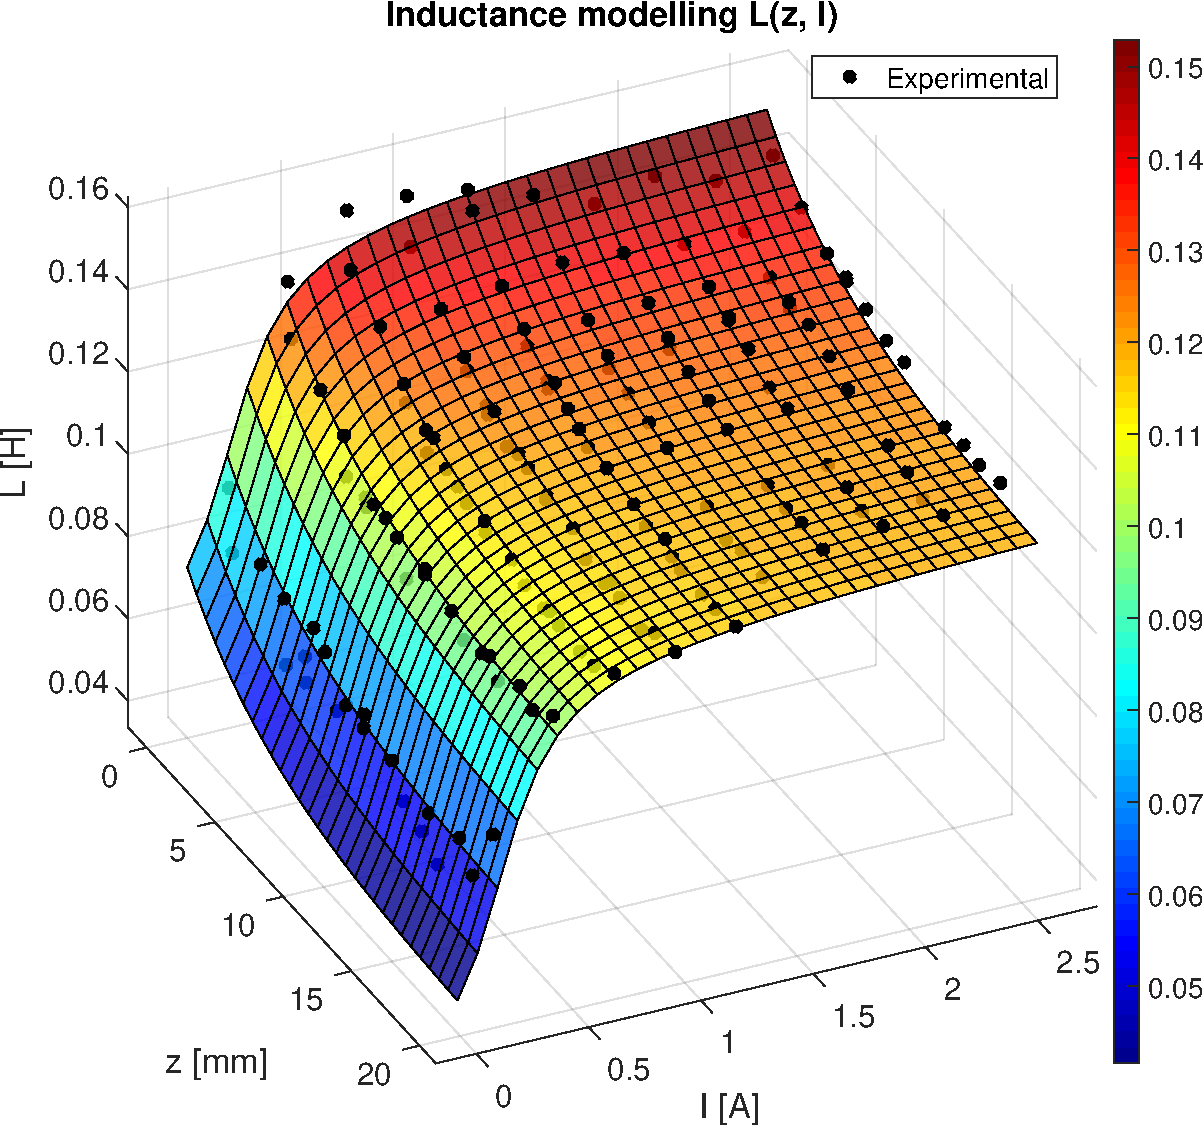
\includegraphics[width=0.6\textwidth]{img/MATLAB/identification/inductance.pdf}
    \caption{Inductance characterization}
    \label{fig:inductance_characterization_inductance}
\end{figure}

One can clearly see the $90$ points that have been used to fit the model proposed in Equation \ref{eq:model_for_inductance} and the obtained fitting.
The values of the parameters are shown in Table \ref{tab:inductance_characterization_parameters}.

\begin{table}[H]
    \centering
    \begin{tabular}{|c|c|c|}
        \hline
        \textbf{Parameter} & \textbf{Value}  & \textbf{Units} \\
        \hline
        $L_0$              & $4.106763e-02$  & $H$            \\
        $a_z$              & $2.155909e+02$  & $1/m$          \\
        $L_z$              & $4.288065e-02$  & $H$            \\
        $a_I$              & $2.553122e+00$  & $1/A$          \\
        $L_I$              & $-7.675453e-02$ & $H$            \\
        \hline
    \end{tabular}

    \caption{Inductance characterization parameters}
    \label{tab:inductance_characterization_parameters}

\end{table}
